\section{Multicore}
Performance steigerung durch Clockfreq. erhöhung (erhöht jedoch Verlustleistung linear - Hitzeprolematik)
\[ P = f_{cl} \cdot C_L \cdot D_{dd}^2 \]
oder Instruktions-Level parallelism (z.B. DSP, Branch prediction wird aufwendig, compiler werden komplex) oder Thread-level parallelism. Bei Thread-Level gibt es die möglichkeit, Uniprocessor durch time-slicing oder mit Mulitprozessoren echte TLP zu erreichen. Dafür muss der Speicher korrekt organisiert werden.

\begin{center}
	\includegraphics[width=\columnwidth]{Images/amdahls}
\end{center}

\subsection{Caches}
Caches führen eine Kopie von häufig benötigten Speicherdaten aus. Im besten Fall sind Daten bereits im Cache vorhanden (Cache Hit). Dann ist es viel schneller als wenn die CPU Daten aus dem Hauptspeicher laden muss (Cache Miss). 
\begin{center}
	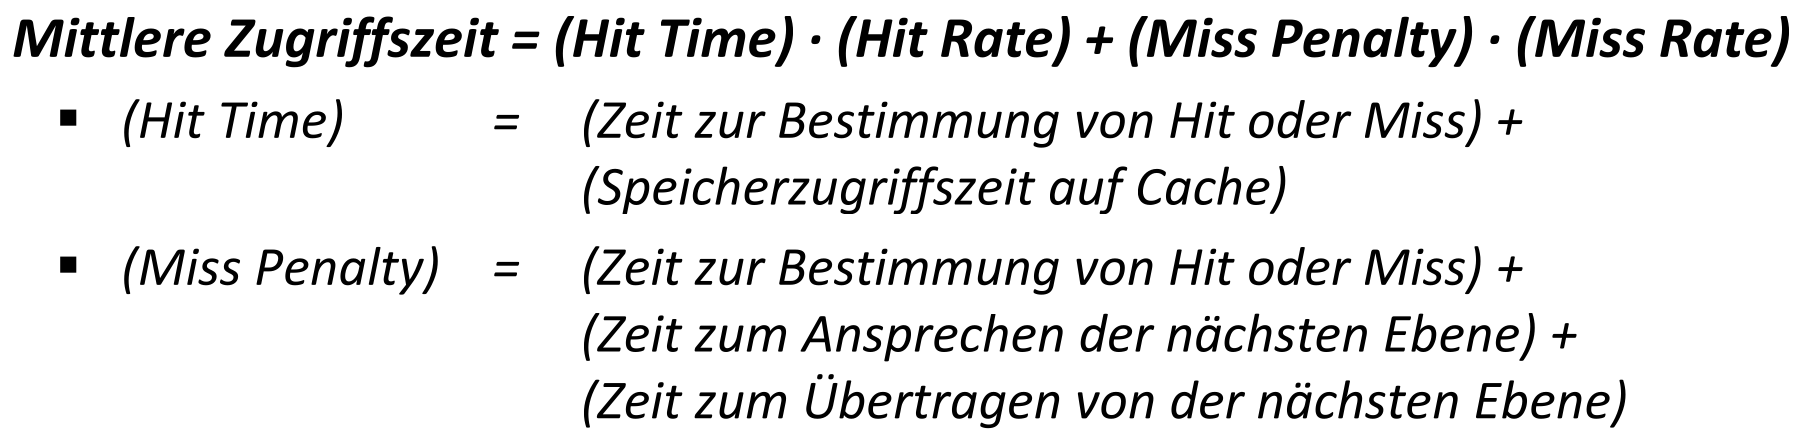
\includegraphics[width=\columnwidth]{Images/mittlerewartezeit}
\end{center}

Als Alternative zur mittleren Wartezeit ist die Worst Case Execution Time (WCET) definiert. Die WCET ist mit einem Cache schlechter als ohne, da zum eigentlichen Zugriff immernoch die Bestimmung ob Hit oder Miss hinzukommt. Ein Cache senkt nur die \textbf{mittlere} Zugriffszeit! Daher sind caches in vielen harten Echtzeitsystem nicht erwünscht.

Um beim laden einer Variable zu verhindern, dass dieser im Cache liegt, muss diese mit dem Keyword \textit{volatile} definiert sein. Dies bewirkt, dass eine CPU die Variable immer frisch aus dem Hauptspeicher liest, und nicht eine Kopie verwendet, was bei Multicore system zu fehlern führen kann.